\chapter{机器人学基础}

\intro{机器人学是研究机器人的设计、制造、控制与应用的学科。作为强化学习在机器人领域应用的基础，本章系统介绍机器人运动学与动力学的核心理论，包括刚体运动的数学描述、DH参数法、雅可比矩阵以及拉格朗日动力学等，为后续章节中强化学习控制方法的应用奠定坚实的理论基础。}

\section{刚体运动的描述}

在机器人学中，我们需要精确描述空间中物体的位置和姿态。一个刚体在三维空间中的位姿（pose）由位置和姿态（orientation）两部分组成，需要用六个独立参数来描述。

\subsection{位置向量}

在三维空间中，一个点的位置可以用一个 $3 \times 1$ 的位置向量来表示。设参考坐标系为 $\{O\}$，点 $P$ 在该坐标系中的坐标为 $(p_x, p_y, p_z)$，则位置向量为：

\begin{myformula}
\mathbf{p} = \begin{bmatrix} p_x \\ p_y \\ p_z \end{bmatrix} \in \R^3
\end{myformula}

位置向量的描述是平凡的，但对于姿态的描述则需要引入旋转矩阵的概念。

\subsection{旋转矩阵与SO(3)}

设刚体上固连一个坐标系 $\{B\}$，其三个坐标轴的单位方向向量在世界坐标系 $\{W\}$ 中分别为 $\mathbf{x}_B, \mathbf{y}_B, \mathbf{z}_B$。则刚体相对于世界坐标系的姿态可以由旋转矩阵表示：

\begin{mydefinition}{旋转矩阵}
一个 $3 \times 3$ 矩阵 $\mathbf{R}$ 被称为旋转矩阵，当且仅当它满足以下两个条件：
\begin{enumerate}
    \item 正交性：$\mathbf{R}^{\T}\mathbf{R} = \mathbf{I}_3$
    \item 行列式为 $+1$：$\det(\mathbf{R}) = +1$
\end{enumerate}
所有旋转矩阵构成的集合称为三维特殊正交群（Special Orthogonal Group），记作 $\mathrm{SO}(3)$：
\begin{myformula}
\mathrm{SO}(3) = \{\mathbf{R} \in \R^{3 \times 3} \mid \mathbf{R}^{\T}\mathbf{R} = \mathbf{I}_3,\ \det(\mathbf{R}) = +1\}
\end{myformula}
\end{mydefinition}

旋转矩阵 $\mathbf{R} = [\mathbf{x}_B \ \mathbf{y}_B \ \mathbf{z}_B]$ 的每一列分别表示坐标系 $\{B\}$ 的坐标轴在参考坐标系中的方向向量。旋转矩阵具有以下重要性质：

\begin{itemize}
    \item 逆等于转置：$\mathbf{R}^{-1} = \mathbf{R}^{\T}$
    \item 保距性：$\|\mathbf{R}\mathbf{v}\| = \|\mathbf{v}\|$，即旋转不改变向量的长度
    \item 保角性：$(\mathbf{R}\mathbf{u})^{\T}(\mathbf{R}\mathbf{v}) = \mathbf{u}^{\T}\mathbf{v}$
    \item 复合旋转：先绕 $\mathbf{R}_1$ 旋转再绕 $\mathbf{R}_2$ 旋转等价于 $\mathbf{R}_2\mathbf{R}_1$
\end{itemize}

\subsection{绕坐标轴的基本旋转}

绕三个坐标轴旋转角度 $\theta$ 的基本旋转矩阵分别为：

\begin{myformula}
\begin{aligned}
\mathbf{R}_x(\theta) &= \begin{bmatrix} 1 & 0 & 0 \\ 0 & \cos\theta & -\sin\theta \\ 0 & \sin\theta & \cos\theta \end{bmatrix} \\[6pt]
\mathbf{R}_y(\theta) &= \begin{bmatrix} \cos\theta & 0 & \sin\theta \\ 0 & 1 & 0 \\ -\sin\theta & 0 & \cos\theta \end{bmatrix} \\[6pt]
\mathbf{R}_z(\theta) &= \begin{bmatrix} \cos\theta & -\sin\theta & 0 \\ \sin\theta & \cos\theta & 0 \\ 0 & 0 & 1 \end{bmatrix}
\end{aligned}
\end{myformula}

这些矩阵可以通过旋转的几何意义直接推导：考虑绕 $z$ 轴旋转时，$z$ 坐标不变，而 $xy$ 平面上的坐标按照二维旋转公式 $(x', y') = (x\cos\theta - y\sin\theta, x\sin\theta + y\cos\theta)$ 变换。

\subsection{齐次变换矩阵与SE(3)}

为了同时描述刚体的位置和姿态，我们引入齐次变换矩阵（Homogeneous Transformation Matrix），它是 $4 \times 4$ 的矩阵：

\begin{mydefinition}{齐次变换矩阵}
\begin{myformula}
\mathbf{T} = \begin{bmatrix} \mathbf{R} & \mathbf{p} \\ \mathbf{0}^{\T} & 1 \end{bmatrix} \in \R^{4 \times 4}
\end{myformula}
其中 $\mathbf{R} \in \mathrm{SO}(3)$ 是旋转矩阵，$\mathbf{p} \in \R^3$ 是位置向量。所有齐次变换矩阵构成三维特殊欧几里得群（Special Euclidean Group），记作 $\mathrm{SE}(3)$。

齐次变换矩阵的逆为：
\begin{myformula}
\mathbf{T}^{-1} = \begin{bmatrix} \mathbf{R}^{\T} & -\mathbf{R}^{\T}\mathbf{p} \\ \mathbf{0}^{\T} & 1 \end{bmatrix}
\end{myformula}
\end{mydefinition}

利用齐次变换矩阵，我们可以方便地实现坐标变换的链式组合。连续应用多个齐次变换对应于矩阵的连乘：
\begin{myformula}
\mathbf{T}_{\text{total}} = \mathbf{T}_1 \mathbf{T}_2 \cdots \mathbf{T}_n
\end{myformula}

\begin{example}
考虑一个坐标系 $\{B\}$，其原点在参考坐标系 $\{A\}$ 的 $(2, 1, 0)$ 处，且 $\{B\}$ 绕 $\{A\}$ 的 $z$ 轴旋转了 $30^\circ$。该变换的齐次变换矩阵为：
\begin{myformula}
^A_B\mathbf{T} = \begin{bmatrix}
\cos 30^\circ & -\sin 30^\circ & 0 & 2 \\
\sin 30^\circ & \cos 30^\circ & 0 & 1 \\
0 & 0 & 1 & 0 \\
0 & 0 & 0 & 1
\end{bmatrix}
\end{myformula}

若点 $P$ 在 $\{B\}$ 中的坐标为 $^B\mathbf{p} = [1, 0, 0]^{\T}$，则其在 $\{A\}$ 中的坐标为：
\begin{myformula}
^A\mathbf{p} = ^A_B\mathbf{T} \cdot ^B\mathbf{p}
\end{myformula}
其中 $^B\mathbf{p}$ 需要扩展为齐次坐标 $[1, 0, 0, 1]^{\T}$。
\end{example}

\subsection{欧拉角}

虽然旋转矩阵提供了姿态的完整描述，但它需要 9 个参数（有 6 个冗余约束）。在实际应用中，我们通常使用更紧凑的表示——欧拉角。

\subsubsection{ZYX欧拉角（Roll-Pitch-Yaw）}

最常见的欧拉角约定是按 $ZYX$ 顺序旋转：先绕 $z$ 轴旋转 $\psi$（Yaw，偏航角），再绕新的 $y'$ 轴旋转 $\theta$（Pitch，俯仰角），最后绕新的 $x''$ 轴旋转 $\phi$（Roll，翻滚角）。对应的旋转矩阵为：

\begin{myformula}
\begin{aligned}
\mathbf{R}_{ZYX}(\phi, \theta, \psi) &= \mathbf{R}_z(\psi)\mathbf{R}_y(\theta)\mathbf{R}_x(\phi) \\
&= \begin{bmatrix}
c_\psi c_\theta & c_\psi s_\theta s_\phi - s_\psi c_\phi & c_\psi s_\theta c_\phi + s_\psi s_\phi \\
s_\psi c_\theta & s_\psi s_\theta s_\phi + c_\psi c_\phi & s_\psi s_\theta c_\phi - c_\psi s_\phi \\
-s_\theta & c_\theta s_\phi & c_\theta c_\phi
\end{bmatrix}
\end{aligned}
\end{myformula}

其中 $c_\theta = \cos\theta$，$s_\theta = \sin\theta$。

\subsubsection{从旋转矩阵到欧拉角}

给定旋转矩阵 $\mathbf{R} = [r_{ij}]$，当 $r_{31} \neq \pm 1$ 时，欧拉角可以通过以下公式反算：

\begin{myformula}
\begin{aligned}
\theta &= \arctan2(-r_{31}, \sqrt{r_{11}^2 + r_{21}^2}) \\
\phi &= \arctan2(r_{32}, r_{33}) \\
\psi &= \arctan2(r_{21}, r_{11})
\end{aligned}
\end{myformula}

\subsubsection{万向节死锁}

当 $\theta = \pm 90^\circ$ 时（即 $r_{31} = \pm 1$），上述反算公式失效，因为此时第一次和第三次旋转轴共线，导致失去一个自由度。这种现象被称为万向节死锁（Gimbal Lock），这是欧拉角表示的一个根本性缺陷。

\begin{remark}
欧拉角表示的三个主要问题：(1) 万向节死锁；(2) 表示不唯一——多种欧拉角可以对应同一个旋转矩阵；(3) 插值不便。替代方案包括四元数（quaternion）和轴角表示（axis-angle），它们在计算机图形学和机器人学中广泛使用。
\end{remark}

\begin{figure}[htbp]
\centering
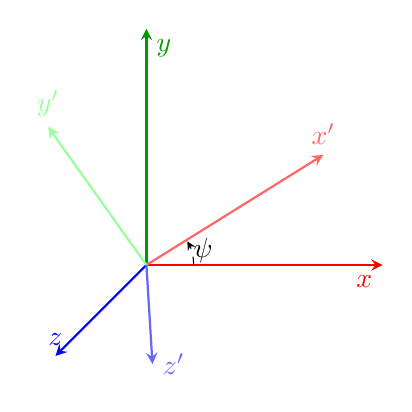
\begin{tikzpicture}[scale=1.2,>=stealth]
    % 绘制三个坐标轴
    \draw[->,thick,red] (0,0,0) -- (2.5,0,0) node[anchor=north east]{$x$};
    \draw[->,thick,green!60!black] (0,0,0) -- (0,2.5,0) node[anchor=north west]{$y$};
    \draw[->,thick,blue] (0,0,0) -- (0,0,2.5) node[anchor=south]{$z$};
    
    % 绘制旋转后的坐标系
    \begin{scope}[rotate around z=30, rotate around y=15, rotate around x=20]
        \draw[->,thick,red!60!white] (0,0,0) -- (2,0,0) node[anchor=south]{$x'$};
        \draw[->,thick,green!40!white] (0,0,0) -- (0,2,0) node[anchor=south]{$y'$};
        \draw[->,thick,blue!60!white] (0,0,0) -- (0,0,2) node[anchor=west]{$z'$};
    \end{scope}
    
    % 标注欧拉角
    \draw[->,dashed] (0.5,0,0) arc (0:30:0.5);
    \node at (0.6,0.15,0) {$\psi$};
\end{tikzpicture}
\caption{绕轴的旋转与欧拉角示意。红色/绿色/蓝色分别表示 $x$/$y$/$z$ 轴，淡色为旋转后的坐标系。}
\label{fig:euler_angles}
\end{figure}

\subsection{四元数表示}

四元数（Quaternion）是姿态表示的另一种重要方法，尤其适用于避免万向节死锁和进行平滑插值。一个四元数定义为：

\begin{mydefinition}{四元数}
\begin{myformula}
\mathbf{q} = q_w + q_x \mathbf{i} + q_y \mathbf{j} + q_z \mathbf{k} = \begin{bmatrix} q_w \\ \mathbf{q}_v \end{bmatrix}
\end{myformula}
其中 $q_w$ 是标量部分，$\mathbf{q}_v = [q_x, q_y, q_z]^{\T}$ 是向量部分。单位四元数满足 $\|\mathbf{q}\| = 1$，用于表示旋转。
\end{mydefinition}

绕单位轴 $\hat{\mathbf{k}}$ 旋转角度 $\theta$ 对应的单位四元数为：
\begin{myformula}
\mathbf{q} = \cos\frac{\theta}{2} + \hat{\mathbf{k}} \sin\frac{\theta}{2}
\end{myformula}

四元数到旋转矩阵的转换公式为：
\begin{myformula}
\mathbf{R} = \begin{bmatrix}
1 - 2q_y^2 - 2q_z^2 & 2q_xq_y - 2q_wq_z & 2q_xq_z + 2q_wq_y \\
2q_xq_y + 2q_wq_z & 1 - 2q_x^2 - 2q_z^2 & 2q_yq_z - 2q_wq_x \\
2q_xq_z - 2q_wq_y & 2q_yq_z + 2q_wq_x & 1 - 2q_x^2 - 2q_y^2
\end{bmatrix}
\end{myformula}

\begin{remark}
四元数的主要优势：(1) 无奇异性，避免了万向节死锁；(2) 通过球面线性插值（SLERP）可实现平滑的旋转插值；(3) 计算效率高，只需要 4 个参数。在强化学习中使用四元数表示姿态时需要注意：$\mathbf{q}$ 和 $-\mathbf{q}$ 表示同一个旋转，这可能导致状态空间的二义性问题。实践中常将四元数映射到 6D 连续表示来解决这个问题，即在状态中使用旋转矩阵的前两列 $[\mathbf{r}_1, \mathbf{r}_2]$。
\end{remark}

\section{DH参数法}

Denavit-Hartenberg（DH）参数法是描述机器人运动学结构的标准方法，由 Jacques Denavit 和 Richard Hartenberg 于 1955 年提出。它为任意串联机械臂提供了一种系统化的连杆坐标系建立方法。

\subsection{DH约定的动机}

串联机械臂由一系列连杆（link）和关节（joint）交替连接而成。DH参数法的核心思想是：用最少的 4 个参数来描述相邻连杆之间的相对位姿关系，从而建立从基座到末端的完整运动学模型。

\subsection{四个DH参数}

对于由关节 $i$ 连接的连杆 $i-1$ 和连杆 $i$，四个DH参数定义如下：

\begin{mydefinition}{标准DH参数}
\begin{itemize}
    \item \textbf{连杆长度} $a_i$：沿 $x_i$ 轴方向，从 $z_{i-1}$ 到 $z_i$ 的距离（当 $z_{i-1}$ 和 $z_i$ 异面时，沿公垂线方向）
    \item \textbf{连杆扭转角} $\alpha_i$：绕 $x_i$ 轴旋转，从 $z_{i-1}$ 到 $z_i$ 的角度（右手法则）
    \item \textbf{连杆偏置} $d_i$：沿 $z_{i-1}$ 轴方向，从 $x_{i-1}$ 到 $x_i$ 的距离
    \item \textbf{关节角度} $\theta_i$：绕 $z_{i-1}$ 轴旋转，从 $x_{i-1}$ 到 $x_i$ 的角度（右手法则）
\end{itemize}
\end{mydefinition}

对于旋转关节，$\theta_i$ 是关节变量，其余为常数；对于移动关节，$d_i$ 是关节变量，其余为常数。

\begin{figure}[htbp]
\centering
\begin{tikzpicture}[scale=1.5,>=stealth]
    % z_{i-1} axis
    \draw[->,thick,blue] (0,-0.5) -- (0,2.5) node[anchor=east]{$z_{i-1}$};
    
    % x_{i-1} axis
    \draw[->,thick,red] (-0.5,0) -- (2.5,0) node[anchor=north]{$x_{i-1}$};
    
    % z_i axis (offset)
    \draw[->,thick,blue!60!black] (2,1.5) -- (2.5,3.5) node[anchor=west]{$z_i$};
    
    % x_i axis
    \draw[->,thick,red!60!black] (1,1.2) -- (3,1.2) node[anchor=north]{$x_i$};
    
    % Common perpendicular
    \draw[dashed] (0,2) -- (2,1.8);
    
    % a_i distance
    \draw[<->] (0,2.2) -- node[above]{$a_i$} (2,2.1);
    
    % d_i distance
    \draw[<->] (-0.3,0) -- node[left]{$d_i$} (-0.3,2);
    
    % theta_i angle
    \draw[->] (0.6,0) arc (0:15:0.6);
    \node at (0.8,0.1) {$\theta_i$};
    
    % alpha_i angle
    \draw[->] (2.2,2.0) arc (0:25:0.4);
    \node at (2.0,2.3) {$\alpha_i$};
    
    % Joint i-1 and i labels
    \node at (0,-0.8) {关节 $i-1$};
    \node at (2.3,3.8) {关节 $i$};
    
    % Origin labels
    \fill (0,0) circle (0.03) node[below left]{$O_{i-1}$};
    \fill (2,1.5) circle (0.03) node[above right]{$O_i$};
\end{tikzpicture}
\caption{DH参数几何示意图。$a_i$ 是沿 $x_i$ 轴的连杆长度，$\alpha_i$ 是绕 $x_i$ 轴的扭转角，$d_i$ 是沿 $z_{i-1}$ 轴的偏置，$\theta_i$ 是绕 $z_{i-1}$ 轴的关节角。}
\label{fig:dh_params}
\end{figure}

\subsection{连杆坐标系的建立规则}

标准DH方法建立坐标系的步骤为（以关节 $i$ 为例）：

\begin{myalgorithm}{标准DH坐标系建立步骤}
\begin{enumerate}
    \item \textbf{确定 $z_{i-1}$ 轴}：沿关节 $i$ 的轴线方向。对于旋转关节，$z_{i-1}$ 是关节的旋转轴；对于移动关节，$z_{i-1}$ 是移动方向。
    \item \textbf{确定原点 $O_{i-1}$}：位于 $z_{i-1}$ 轴和 $z_i$ 轴的公垂线与 $z_{i-1}$ 轴的交点处。若两轴平行，则原点可任意选择；若两轴相交，原点选在交点。
    \item \textbf{确定 $x_{i-1}$ 轴}：沿 $z_{i-1}$ 轴到 $z_i$ 轴的公垂线方向，指向 $z_i$ 轴。若两轴平行，选择使 $d_i = 0$ 的方向（很多选择）。
    \item \textbf{确定 $y_{i-1}$ 轴}：按右手定则确定：$\mathbf{y}_{i-1} = \mathbf{z}_{i-1} \times \mathbf{x}_{i-1}$。
    \item \textbf{基座坐标系 $\{0\}$}：为方便，常选择与 $\{1\}$ 在 $\theta_1 = 0$ 时重合。
    \item \textbf{末端坐标系 $\{n\}$}：常选择与 $\{n-1\}$ 在对齐位置时重合，$x_n$ 轴方向任意。
\end{enumerate}
\end{myalgorithm}

\subsection{DH变换矩阵的推导}

坐标系 $\{i\}$ 可以通过以下四步变换从坐标系 $\{i-1\}$ 得到：

\begin{enumerate}
    \item 绕 $z_{i-1}$ 轴旋转 $\theta_i$：$\mathrm{Rot}(z_{i-1}, \theta_i)$
    \item 沿 $z_{i-1}$ 轴平移 $d_i$：$\mathrm{Trans}(z_{i-1}, d_i)$
    \item 沿 $x_i$ 轴平移 $a_i$：$\mathrm{Trans}(x_i, a_i)$
    \item 绕 $x_i$ 轴旋转 $\alpha_i$：$\mathrm{Rot}(x_i, \alpha_i)$
\end{enumerate}

将这四个基本变换连乘，得到单个连杆的DH变换矩阵：

\begin{myformula}
\begin{aligned}
^{i-1}_i\mathbf{T} &= \mathbf{R}_z(\theta_i) \cdot \mathbf{T}_z(d_i) \cdot \mathbf{T}_x(a_i) \cdot \mathbf{R}_x(\alpha_i) \\[6pt]
&= \begin{bmatrix}
\cos\theta_i & -\sin\theta_i\cos\alpha_i & \sin\theta_i\sin\alpha_i & a_i\cos\theta_i \\[3pt]
\sin\theta_i & \cos\theta_i\cos\alpha_i & -\cos\theta_i\sin\alpha_i & a_i\sin\theta_i \\[3pt]
0 & \sin\alpha_i & \cos\alpha_i & d_i \\[3pt]
0 & 0 & 0 & 1
\end{bmatrix}
\end{aligned}
\end{myformula}

\subsection{标准DH vs 改进DH}

改进DH（Modified DH，又称Craig DH）与标准DH的主要区别在于坐标系的放置位置：

\begin{itemize}
    \item \textbf{标准DH}：坐标系 $\{i\}$ 固连在连杆 $i$ 的远端（靠近关节 $i+1$ 处）
    \item \textbf{改进DH}：坐标系 $\{i\}$ 固连在连杆 $i$ 的近端（靠近关节 $i$ 处）
\end{itemize}

改进DH的变换公式为：
\begin{myformula}
^{i-1}_i\mathbf{T}_{\text{MDH}} = \mathbf{R}_x(\alpha_{i-1}) \cdot \mathbf{T}_x(a_{i-1}) \cdot \mathbf{R}_z(\theta_i) \cdot \mathbf{T}_z(d_i)
\end{myformula}

\begin{remark}
在实际工程中，标准DH更适合描述树形结构机器人，改进DH更适合描述串联机器人。URDF（Unified Robot Description Format）文件格式使用改进DH约定。在ROS和MuJoCo等仿真环境中，需要特别注意所使用的DH约定版本。
\end{remark}

\subsection{完整示例：平面2R机械臂}

考虑一个在平面内运动的双连杆机械臂（2R平面臂）。两个旋转关节的轴线均垂直于运动平面。

\begin{figure}[htbp]
\centering
\begin{tikzpicture}[scale=1.8,>=stealth]
    % Base
    \fill[gray!50] (-0.3,-0.3) rectangle (0.3,0);
    \draw[thick] (-0.3,0) -- (0.3,0);
    
    % Joint 1
    \fill (0,0) circle (0.05);
    \node[below] at (0,0) {关节1};
    
    % Link 1
    \draw[very thick,blue!70!black] (0,0) -- (1.5,0.8);
    
    % Joint 2
    \fill (1.5,0.8) circle (0.05);
    \node[right] at (1.5,0.8) {关节2};
    
    % Link 2
    \draw[very thick,red!70!black] (1.5,0.8) -- (2.8,0.2);
    
    % End-effector
    \fill (2.8,0.2) circle (0.05);
    \node[right] at (2.8,0.2) {末端};
    
    % Angles
    \draw[->] (0.6,0) arc (0:28:0.6);
    \node at (0.8,0.2) {$\theta_1$};
    
    \draw[->] (1.5,0.8) ++(-30:0.6) arc (-30:-55:0.6);
    \node at (2.0,0.35) {$\theta_2$};
    
    % Lengths
    \node[blue] at (0.7,0.5) {$l_1$};
    \node[red] at (2.2,0.6) {$l_2$};
    
    % Coordinate frame at base
    \draw[->] (-0.5,0) -- (0.5,0) node[below]{$x_0$};
    \draw[->] (0,-0.5) -- (0,0.5) node[left]{$y_0$};
    
    % Dashed lines
    \draw[dashed] (1.5,0.8) -- (1.5,0);
    \draw[dashed] (2.8,0.2) -- (2.8,-0.2);
\end{tikzpicture}
\caption{平面2R机械臂示意图。两个旋转关节的轴线均垂直于纸面，连杆长度分别为 $l_1$ 和 $l_2$，关节角度分别为 $\theta_1$ 和 $\theta_2$。}
\label{fig:2r_arm}
\end{figure}

\subsubsection{DH参数表}

平面2R臂的DH参数如表~\ref{tab:2r_dh}所示：

\begin{table}[htbp]
\centering
\caption{平面2R臂的DH参数表}
\label{tab:2r_dh}
\begin{tabular}{ccccc}
\toprule
连杆 $i$ & $\alpha_i$ & $a_i$ & $d_i$ & $\theta_i$ \\
\midrule
1 & 0 & $l_1$ & 0 & $\theta_1$ \\
2 & 0 & $l_2$ & 0 & $\theta_2$ \\
\bottomrule
\end{tabular}
\end{table}

\subsubsection{单个连杆变换矩阵}

\begin{myformula}
^0_1\mathbf{T} = \begin{bmatrix}
\cos\theta_1 & -\sin\theta_1 & 0 & l_1\cos\theta_1 \\
\sin\theta_1 & \cos\theta_1 & 0 & l_1\sin\theta_1 \\
0 & 0 & 1 & 0 \\
0 & 0 & 0 & 1
\end{bmatrix}, \qquad
^1_2\mathbf{T} = \begin{bmatrix}
\cos\theta_2 & -\sin\theta_2 & 0 & l_2\cos\theta_2 \\
\sin\theta_2 & \cos\theta_2 & 0 & l_2\sin\theta_2 \\
0 & 0 & 1 & 0 \\
0 & 0 & 0 & 1
\end{bmatrix}
\end{myformula}

\subsubsection{正运动学解}

\begin{myformula}
^0_2\mathbf{T} = ^0_1\mathbf{T} \cdot ^1_2\mathbf{T} = \begin{bmatrix}
\cos(\theta_1+\theta_2) & -\sin(\theta_1+\theta_2) & 0 & l_1\cos\theta_1 + l_2\cos(\theta_1+\theta_2) \\
\sin(\theta_1+\theta_2) & \cos(\theta_1+\theta_2) & 0 & l_1\sin\theta_1 + l_2\sin(\theta_1+\theta_2) \\
0 & 0 & 1 & 0 \\
0 & 0 & 0 & 1
\end{bmatrix}
\end{myformula}

末端执行器的位置为：
\begin{myformula}
\begin{aligned}
x &= l_1\cos\theta_1 + l_2\cos(\theta_1 + \theta_2) \\
y &= l_1\sin\theta_1 + l_2\sin(\theta_1 + \theta_2)
\end{aligned}
\end{myformula}

\subsection{PUMA 560 机器人}

PUMA 560 是经典的六自由度工业机器人，其DH参数如表~\ref{tab:puma_dh}所示：

\begin{table}[htbp]
\centering
\caption{PUMA 560的DH参数表}
\label{tab:puma_dh}
\begin{tabular}{ccccc}
\toprule
$i$ & $\alpha_i$ (rad) & $a_i$ (m) & $d_i$ (m) & $\theta_i$ \\
\midrule
1 & 0 & 0 & 0 & $\theta_1$ \\
2 & $-\pi/2$ & 0 & 0 & $\theta_2$ \\
3 & 0 & $a_2$ & $d_3$ & $\theta_3$ \\
4 & $-\pi/2$ & $a_3$ & $d_4$ & $\theta_4$ \\
5 & $\pi/2$ & 0 & 0 & $\theta_5$ \\
6 & $-\pi/2$ & 0 & 0 & $\theta_6$ \\
\bottomrule
\end{tabular}
\end{table}

其中典型的连杆参数为：$a_2 = 0.4318$m, $a_3 = -0.0203$m, $d_3 = 0.1500$m, $d_4 = 0.4318$m。

\begin{remark}
现代机器人学实践中，除了DH参数法，还常使用\textbf{乘积形式指数（Product of Exponentials, PoE）}表示法，它基于旋量理论（Screw Theory），避免了DH参数法中当关节轴平行或接近平行时的奇异问题。PoE方法直接通过定义基座坐标系和末端工具坐标系，以及各关节的旋量坐标来描述运动学，具有更好的数值稳定性和更简洁的数学表达。
\end{remark}

\section{正运动学}

正运动学（Forward Kinematics）是指给定各关节的关节变量（旋转关节的角度或移动关节的位移），计算末端执行器相对于基座坐标系的位姿。

\subsection{变换矩阵连乘}

对于具有 $n$ 个关节的串联机器人，从基座坐标系 $\{0\}$ 到末端坐标系 $\{n\}$ 的齐次变换矩阵为各连杆变换矩阵的乘积：

\begin{myformula}
^0_n\mathbf{T}(\mathbf{q}) = ^0_1\mathbf{T}(q_1) \cdot ^1_2\mathbf{T}(q_2) \cdot \cdots \cdot {}^{n-1}_n\mathbf{T}(q_n)
\end{myformula}

其中 $\mathbf{q} = [q_1, q_2, \ldots, q_n]^{\T}$ 是关节变量向量，$^0_n\mathbf{T}$ 的结构为：
\begin{myformula}
^0_n\mathbf{T} = \begin{bmatrix}
\mathbf{r}_{11} & \mathbf{r}_{12} & \mathbf{r}_{13} & p_x \\
\mathbf{r}_{21} & \mathbf{r}_{22} & \mathbf{r}_{23} & p_y \\
\mathbf{r}_{31} & \mathbf{r}_{32} & \mathbf{r}_{33} & p_z \\
0 & 0 & 0 & 1
\end{bmatrix} = \begin{bmatrix}
^0_n\mathbf{R} & ^0\mathbf{p}_n \\
\mathbf{0}^{\T} & 1
\end{bmatrix}
\end{myformula}

其中 $^0_n\mathbf{R}$ 是末端坐标系相对于基座的旋转矩阵，$^0\mathbf{p}_n$ 是末端原点在基坐标系中的位置向量。具体地，$^0\mathbf{p}_n = [p_x, p_y, p_z]^{\T}$ 和 $^0_n\mathbf{R}$ 分别给出了末端执行器的位置和姿态。这六个量中只有三个是位置独立的，加上姿态的三个自由度，末端执行器的位姿总共有六个自由度。

\subsection{末端位姿的计算}

在实际编程实现中，正运动学可以通过迭代方式高效计算：对于 $i = 1$ 到 $n$，逐个连乘变换矩阵。最终结果可以直接提取位置坐标和姿态（欧拉角或四元数）。

\begin{myalgorithm}{正运动学迭代算法}
\begin{enumerate}
    \item 初始化 $\mathbf{T} = \mathbf{I}_4$
    \item 对于 $i = 1, 2, \ldots, n$：
    \begin{itemize}
        \item 计算 $^{i-1}_i\mathbf{T}$ 使用DH变换公式
        \item $\mathbf{T} \leftarrow \mathbf{T} \cdot {}^{i-1}_i\mathbf{T}$
    \end{itemize}
    \item 从 $\mathbf{T}$ 中提取位置 $\mathbf{p}$ 和旋转矩阵 $\mathbf{R}$
\end{enumerate}
\end{myalgorithm}

\section{雅可比矩阵}

雅可比矩阵（Jacobian）描述了关节速度与末端执行器速度之间的线性映射关系，是机器人速度运动学和控制的核心工具。

\subsection{速度运动学}

末端执行器的速度（即所谓"twist"，由线速度和角速度组成）可以由一个 $6 \times 1$ 的向量表示：
\begin{myformula}
\boldsymbol{\nu}_e = \begin{bmatrix} \mathbf{v}_e \\ \boldsymbol{\omega}_e \end{bmatrix} \in \R^6
\end{myformula}

其中 $\mathbf{v}_e \in \R^3$ 是末端在基坐标系中的线速度，$\boldsymbol{\omega}_e \in \R^3$ 是末端的角速度。

雅可比矩阵建立了关节速度 $\dot{\mathbf{q}}$ 和末端速度 $\boldsymbol{\nu}_e$ 之间的线性关系：

\begin{mydefinition}{雅可比矩阵}
\begin{myformula}
\boldsymbol{\nu}_e = \mathbf{J}(\mathbf{q}) \dot{\mathbf{q}}, \qquad 
\mathbf{J}(\mathbf{q}) \in \R^{6 \times n}
\end{myformula}
其中 $\mathbf{J}(\mathbf{q})$ 是依赖于当前关节构型的雅可比矩阵，通常写为分块形式：
\begin{myformula}
\boldsymbol{\nu}_e = \begin{bmatrix} \mathbf{J}_v(\mathbf{q}) \\ \mathbf{J}_\omega(\mathbf{q}) \end{bmatrix} \dot{\mathbf{q}}
\end{myformula}
$\mathbf{J}_v$ 和 $\mathbf{J}_\omega$ 分别是位置雅可比和姿态雅可比，各为 $3 \times n$ 矩阵。
\end{mydefinition}

\subsection{几何雅可比}

几何雅可比（Geometric Jacobian）直接从运动学几何关系推导，以末端线速度和角速度（在基坐标系中表示）为输出。

对于第 $i$ 个关节（假设为旋转关节），它对末端线速度和角速度的贡献为：

\begin{myformula}
\begin{aligned}
\mathbf{J}_{v,i} &= \mathbf{z}_{i-1} \times (\mathbf{p}_n - \mathbf{p}_{i-1}) \\[3pt]
\mathbf{J}_{\omega,i} &= \mathbf{z}_{i-1}
\end{aligned}
\end{myformula}

其中 $\mathbf{z}_{i-1}$ 是关节 $i$ 的旋转轴在基坐标系中的方向向量，$\mathbf{p}_{i-1}$ 是坐标系 $\{i-1\}$ 原点的位置，$\mathbf{p}_n$ 是末端原点的位置。这里 $\mathbf{z}_{i-1}$ 和 $\mathbf{p}_{i-1}$ 可以通过正运动学从基座到第 $i-1$ 个连杆的变换矩阵 $^0_{i-1}\mathbf{T}$ 中提取。

\textbf{推导}：旋转关节 $i$ 以角速度 $\dot{q}_i$ 绕轴 $\mathbf{z}_{i-1}$ 旋转，该旋转使末端执行器产生绕 $\mathbf{z}_{i-1}$ 轴的角速度 $\dot{q}_i \mathbf{z}_{i-1}$，同时使末端以线速度 $\dot{q}_i \mathbf{z}_{i-1} \times (\mathbf{p}_n - \mathbf{p}_{i-1})$ 运动。

对于移动关节，其贡献为：
\begin{myformula}
\mathbf{J}_{v,i} = \mathbf{z}_{i-1}, \qquad \mathbf{J}_{\omega,i} = \mathbf{0}
\end{myformula}

完整雅可比矩阵按列组装：
\begin{myformula}
\mathbf{J}(\mathbf{q}) = \begin{bmatrix}
\mathbf{J}_1 & \mathbf{J}_2 & \cdots & \mathbf{J}_n
\end{bmatrix}
\end{myformula}

\begin{figure}[htbp]
\centering
\begin{tikzpicture}[scale=1.3,>=stealth]
    % Base
    \fill[gray!50] (-0.2,-0.2) rectangle (0.2,0);
    \draw[thick] (-0.2,0) -- (0.2,0);
    
    % Joint axes (coming out of plane)
    \node[circle,draw,inner sep=0pt,minimum size=6pt,fill=black] (j1) at (0,0) {};
    \node[circle,draw,inner sep=0pt,minimum size=6pt,fill=black] (j2) at (2,1) {};
    \node[circle,draw,inner sep=0pt,minimum size=6pt,fill=black] (ee) at (3.5,0.8) {};
    
    % Links
    \draw[thick,blue!70!black] (j1) -- (j2);
    \draw[thick,red!70!black] (j2) -- (ee);
    
    % z axes (out of plane - circle with dot)
    \node at (0,0.4) {$\mathbf{z}_0 \odot$};
    \node at (2,1.4) {$\mathbf{z}_1 \odot$};
    
    % Velocity vectors
    \draw[->,very thick,green!50!black] (j2) -- (3.0,0.5) node[midway,right]{$\dot{\theta}_1 \mathbf{z}_0 \times \mathbf{r}_1$};
    \draw[->,very thick,green!50!black] (ee) -- (4.3,1.6) node[midway,right]{$\dot{\theta}_2 \mathbf{z}_1 \times \mathbf{r}_2$};
    
    % Resultant
    \draw[->,very thick,orange] (ee) -- (4.5,1.0) node[right]{$\mathbf{v}_e$};
    
    % r vectors
    \draw[dashed] (j1) -- (j2);
    \draw[dashed] (j1) -- (ee);
    \node at (1,0.2) {$\mathbf{r}_1$};
    \node at (2.8,1.1) {$\mathbf{r}_2$};
    
    % Labels
    \node[below] at (0,-0.1) {$\theta_1$};
    \node[right] at (2,0.9) {$\theta_2$};
    \node[above] at (ee) {末端};
\end{tikzpicture}
\caption{旋转关节对末端速度贡献的几何示意。关节 $i$ 的旋转产生末端线速度 $\dot{\theta}_i (\mathbf{z}_{i-1} \times \mathbf{r}_i)$，其中 $\mathbf{r}_i = \mathbf{p}_n - \mathbf{p}_{i-1}$。}
\label{fig:jacobian_geom}
\end{figure}

\subsection{解析雅可比}

解析雅可比（Analytical Jacobian）描述的是关节速度与末端执行器\textit{位姿参数}变化率之间的关系。如果我们用最小参数 $\mathbf{x} \in \R^m$（例如，3个位置 + 3个欧拉角）来描述末端位姿，则：

\begin{myformula}
\dot{\mathbf{x}} = \mathbf{J}_A(\mathbf{q}) \dot{\mathbf{q}}
\end{myformula}

解析雅可比与几何雅可比的关系为：
\begin{myformula}
\mathbf{J}_A(\mathbf{q}) = \mathbf{E}(\mathbf{x})^{-1} \mathbf{J}(\mathbf{q})
\end{myformula}

其中 $\mathbf{E}(\mathbf{x})$ 是将角速度映射为姿态参数变化率的变换矩阵，依赖于所使用的姿态参数化方式。对于 ZYX 欧拉角 $\boldsymbol{\phi} = [\phi, \theta, \psi]^{\T}$：

\begin{myformula}
\mathbf{E}(\boldsymbol{\phi}) = \begin{bmatrix}
\cos\theta\cos\psi & -\sin\psi & 0 \\
\cos\theta\sin\psi & \cos\psi & 0 \\
-\sin\theta & 0 & 1
\end{bmatrix}
\end{myformula}

\subsection{奇异性}

奇异性（Singularity）是指机器人在某些构型下雅可比矩阵 $\mathbf{J}(\mathbf{q})$ 降秩的情况，即：
\begin{myformula}
\det(\mathbf{J}(\mathbf{q})) = 0 \quad \text{(对正方雅可比)} \quad \text{或} \quad \operatorname{rank}(\mathbf{J}(\mathbf{q})) < \min(6, n)
\end{myformula}

奇异构型的物理表现包括：
\begin{itemize}
    \item \textbf{工作空间边界奇异}：机器人完全伸展或收拢，无法在某个方向上产生运动
    \item \textbf{工作空间内部奇异}：两个或多个关节轴共线，导致失去一个运动自由度
    \item \textbf{腕部奇异}：末端三个关节轴共面，常见于球腕结构
\end{itemize}

在奇异构型附近，微小的末端速度变化需要极大的关节速度来实现，这在控制中可能导致不稳定甚至危险。在强化学习控制中，通常需要加入正则化项来惩罚接近奇异的构型：

\begin{myformula}
r_{\text{sing}} = -w_{\text{sing}} \cdot \frac{1}{\det(\mathbf{J}\mathbf{J}^{\T}) + \epsilon}
\end{myformula}

\subsection{力域雅可比}

根据虚功原理（Principle of Virtual Work），末端执行器施加的外力/力矩 $\mathbf{F}_e = [\mathbf{f}_e^{\T}, \mathbf{n}_e^{\T}]^{\T}$ 与所需关节力矩 $\boldsymbol{\tau}$ 之间的关系由力域雅可比（Force-Domain Jacobian）给出：

\begin{mydefinition}{力域雅可比——虚功原理}
\begin{myformula}
\boldsymbol{\tau} = \mathbf{J}(\mathbf{q})^{\T} \mathbf{F}_e
\end{myformula}
\end{mydefinition}

\textbf{推导}：根据虚功原理，在外力作用下机器人处于静力平衡时，外力在虚位移上做的虚功等于关节力矩在虚位移上做的虚功：
\begin{myformula}
\boldsymbol{\tau}^{\T} \delta\mathbf{q} = \mathbf{F}_e^{\T} \delta\mathbf{x}
\end{myformula}

利用 $\delta\mathbf{x} = \mathbf{J}\delta\mathbf{q}$，代入得：
\begin{myformula}
\boldsymbol{\tau}^{\T} \delta\mathbf{q} = \mathbf{F}_e^{\T} \mathbf{J} \delta\mathbf{q}
\end{myformula}

由于 $\delta\mathbf{q}$ 是任意的，得到 $\boldsymbol{\tau}^{\T} = \mathbf{F}_e^{\T} \mathbf{J}$，即 $\boldsymbol{\tau} = \mathbf{J}^{\T} \mathbf{F}_e$。

这一关系在基于力和力矩的控制策略以及在强化学习中设计力/力矩相关的奖励函数时非常有用——例如，可以将能耗项直接表达为 $\|\boldsymbol{\tau}\|^2$。

\begin{remark}
雅可比矩阵的两个基本应用：(1) \textbf{速度域} $\boldsymbol{\nu}_e = \mathbf{J}\dot{\mathbf{q}}$——用于运动控制和轨迹跟踪；(2) \textbf{力域} $\boldsymbol{\tau} = \mathbf{J}^{\T}\mathbf{F}_e$——用于力控制和阻抗控制。这种速度-力对偶性是机器人学中最优雅的结构之一，反映了运动学与静力学之间的深层次联系。
\end{remark}

\section{机器人动力学}

机器人动力学研究关节力矩与关节运动（位置、速度、加速度）之间的关系。动力学方程是机器人控制、仿真以及强化学习中动作-状态转换建模的基础。

\subsection{Lagrangian形式的动力学方程}

拉格朗日力学从能量角度出发，通过系统动能 $\mathcal{K}$ 和势能 $\mathcal{P}$ 来推导运动方程。定义拉格朗日量 $\mathcal{L} = \mathcal{K} - \mathcal{P}$，则运动方程为：

\begin{myformula}
\frac{d}{dt}\left(\frac{\partial \mathcal{L}}{\partial \dot{\mathbf{q}}}\right) - \frac{\partial \mathcal{L}}{\partial \mathbf{q}} = \boldsymbol{\tau}
\end{myformula}

对于一般的 $n$ 自由度串联机器人，应用拉格朗日方程可以得到标准形式的动力学方程：

\begin{mydefinition}{机器人动力学方程——标准形式}
\begin{myformula}
\mathbf{M}(\mathbf{q})\ddot{\mathbf{q}} + \mathbf{C}(\mathbf{q}, \dot{\mathbf{q}})\dot{\mathbf{q}} + \mathbf{g}(\mathbf{q}) = \boldsymbol{\tau}
\end{myformula}
其中：
\begin{itemize}
    \item $\mathbf{M}(\mathbf{q}) \in \R^{n \times n}$：惯性矩阵（正定、对称）
    \item $\mathbf{C}(\mathbf{q}, \dot{\mathbf{q}}) \in \R^{n \times n}$：科里奥利力和离心力矩阵
    \item $\mathbf{g}(\mathbf{q}) \in \R^{n}$：重力项
    \item $\boldsymbol{\tau} \in \R^{n}$：关节驱动力/力矩
\end{itemize}
\end{mydefinition}

\subsubsection{各矩阵的物理含义}

\textbf{惯性矩阵 $\mathbf{M}(\mathbf{q})$}：描述了各关节加速度对所需力矩的贡献。$M_{ij}$ 表示第 $j$ 个关节的加速度在第 $i$ 个关节处引起的惯性力矩。$\mathbf{M}(\mathbf{q})$ 具有以下性质：

\begin{itemize}
    \item 正定性：$\mathbf{M}(\mathbf{q}) \succ 0$，对任意 $\mathbf{q}$
    \item 对称性：$\mathbf{M}(\mathbf{q}) = \mathbf{M}(\mathbf{q})^{\T}$
    \item $\dot{\mathbf{M}}(\mathbf{q}) - 2\mathbf{C}(\mathbf{q}, \dot{\mathbf{q}})$ 是反对称矩阵（重要性质，用于证明稳定性）
\end{itemize}

\textbf{科里奥利力和离心力项 $\mathbf{C}(\mathbf{q}, \dot{\mathbf{q}})\dot{\mathbf{q}}$}：描述由于关节运动产生的速度相关力。具体地，科里奥利力来源于不同关节之间的速度耦合，离心力来源于单个关节绕轴旋转时产生的离心效应。

设 $\mathbf{c} = \mathbf{C}\dot{\mathbf{q}}$，其第 $i$ 个分量为：
\begin{myformula}
c_i = \sum_{j=1}^{n} \sum_{k=1}^{n} c_{ijk} \dot{q}_j \dot{q}_k
\end{myformula}

其中 $c_{ijk}$ 称为第一类 Christoffel 符号：
\begin{myformula}
c_{ijk} = \frac{1}{2}\left(\frac{\partial M_{ij}}{\partial q_k} + \frac{\partial M_{ik}}{\partial q_j} - \frac{\partial M_{jk}}{\partial q_i}\right)
\end{myformula}

\textbf{重力项 $\mathbf{g}(\mathbf{q})$}：描述由于重力作用在机器人上产生的关节力矩：
\begin{myformula}
\mathbf{g}(\mathbf{q}) = \frac{\partial \mathcal{P}}{\partial \mathbf{q}}
\end{myformula}

其中 $\mathcal{P}$ 是系统的总重力势能。对于每个连杆，$\mathcal{P}_i = -m_i \mathbf{g}_0^{\T} \mathbf{p}_{c_i}$，这里 $m_i$ 是连杆 $i$ 的质量，$\mathbf{g}_0$ 是重力加速度向量，$\mathbf{p}_{c_i}$ 是连杆 $i$ 质心的位置向量。

\subsection{平面2R臂的Lagrangian动力学}

以平面2R臂为例，应用拉格朗日方法推导动力学方程。设连杆质量为 $m_1, m_2$，长度为 $l_1, l_2$，质心到关节的距离为 $l_{c1}, l_{c2}$，绕质心的转动惯量为 $I_1, I_2$。

\textbf{动能}：
\begin{myformula}
\mathcal{K} = \frac{1}{2}(m_1 l_{c1}^2 + I_1 + m_2 l_1^2)\dot{\theta}_1^2 + \frac{1}{2}(m_2 l_{c2}^2 + I_2)(\dot{\theta}_1 + \dot{\theta}_2)^2 + m_2 l_1 l_{c2} \dot{\theta}_1(\dot{\theta}_1+\dot{\theta}_2)\cos\theta_2
\end{myformula}

\textbf{势能}（取 $y=0$ 平面为零势能面）：
\begin{myformula}
\mathcal{P} = m_1 g l_{c1}\sin\theta_1 + m_2 g (l_1\sin\theta_1 + l_{c2}\sin(\theta_1+\theta_2))
\end{myformula}

应用拉格朗日方程，得到动力学方程的形式为：
\begin{myformula}
\begin{bmatrix} M_{11} & M_{12} \\ M_{21} & M_{22} \end{bmatrix} \begin{bmatrix} \ddot{\theta}_1 \\ \ddot{\theta}_2 \end{bmatrix} + \begin{bmatrix} -h\dot{\theta}_2 & -h(\dot{\theta}_1+\dot{\theta}_2) \\ h\dot{\theta}_1 & 0 \end{bmatrix} \begin{bmatrix} \dot{\theta}_1 \\ \dot{\theta}_2 \end{bmatrix} + \begin{bmatrix} g_1 \\ g_2 \end{bmatrix} = \begin{bmatrix} \tau_1 \\ \tau_2 \end{bmatrix}
\end{myformula}

其中各元素为：
\begin{myformula}
\begin{aligned}
M_{11} &= m_1 l_{c1}^2 + m_2(l_1^2 + l_{c2}^2 + 2l_1l_{c2}\cos\theta_2) + I_1 + I_2 \\
M_{12} &= M_{21} = m_2(l_{c2}^2 + l_1l_{c2}\cos\theta_2) + I_2 \\
M_{22} &= m_2 l_{c2}^2 + I_2 \\
h &= m_2 l_1 l_{c2} \sin\theta_2 \\
g_1 &= (m_1l_{c1} + m_2l_1)g\cos\theta_1 + m_2l_{c2}g\cos(\theta_1+\theta_2) \\
g_2 &= m_2l_{c2}g\cos(\theta_1+\theta_2)
\end{aligned}
\end{myformula}

\subsection{Newton-Euler递推算法}

Newton-Euler（NE）递推算法是一种计算效率极高的动力学算法，其复杂度为 $O(n)$（$n$ 为自由度数），而直接使用 Lagrangian 方法的复杂度为 $O(n^3)$。NE算法分为两步：

\begin{myalgorithm}{Newton-Euler递推算法}
\textbf{正向递推（从基座到末端）}：对于 $i = 1, \ldots, n$，计算每个连杆的速度和加速度。

\begin{enumerate}
    \item 角速度递推：
    \begin{myformula}
    \boldsymbol{\omega}_i = \boldsymbol{\omega}_{i-1} + \dot{q}_i \mathbf{z}_{i-1} \quad \text{(旋转关节)}
    \end{myformula}
    \item 角加速度递推：
    \begin{myformula}
    \dot{\boldsymbol{\omega}}_i = \dot{\boldsymbol{\omega}}_{i-1} + \ddot{q}_i \mathbf{z}_{i-1} + \dot{q}_i \boldsymbol{\omega}_{i-1} \times \mathbf{z}_{i-1}
    \end{myformula}
    \item 线加速度递推：
    \begin{myformula}
    \ddot{\mathbf{p}}_i = \ddot{\mathbf{p}}_{i-1} + \dot{\boldsymbol{\omega}}_i \times \mathbf{r}_i + \boldsymbol{\omega}_i \times (\boldsymbol{\omega}_i \times \mathbf{r}_i)
    \end{myformula}
    \item 质心加速度：
    \begin{myformula}
    \ddot{\mathbf{p}}_{c_i} = \ddot{\mathbf{p}}_i + \dot{\boldsymbol{\omega}}_i \times \mathbf{r}_{c_i} + \boldsymbol{\omega}_i \times (\boldsymbol{\omega}_i \times \mathbf{r}_{c_i})
    \end{myformula}
\end{enumerate}

\textbf{逆向递推（从末端到基座）}：对于 $i = n, \ldots, 1$，计算每个关节的力和力矩。

\begin{enumerate}
    \setcounter{enumi}{4}
    \item 作用在连杆 $i$ 上的力：
    \begin{myformula}
    \mathbf{F}_i = m_i \ddot{\mathbf{p}}_{c_i}
    \end{myformula}
    \item 作用在连杆 $i$ 上的力矩：
    \begin{myformula}
    \mathbf{N}_i = \mathbf{I}_i \dot{\boldsymbol{\omega}}_i + \boldsymbol{\omega}_i \times (\mathbf{I}_i \boldsymbol{\omega}_i)
    \end{myformula}
    \item 力/力矩平衡递推：
    \begin{myformula}
    \begin{aligned}
    \mathbf{f}_i &= \mathbf{F}_i + {}^{i}_{i+1}\mathbf{R}\,\mathbf{f}_{i+1} \\
    \mathbf{n}_i &= \mathbf{N}_i + {}^{i}_{i+1}\mathbf{R}\,\mathbf{n}_{i+1} + \mathbf{r}_{c_i} \times \mathbf{F}_i + \mathbf{r}_{i+1} \times ({}^{i}_{i+1}\mathbf{R}\,\mathbf{f}_{i+1})
    \end{aligned}
    \end{myformula}
    \item 关节力矩（旋转关节）：
    \begin{myformula}
    \tau_i = \mathbf{n}_i^{\T} {}^{i-1}_i\mathbf{R}\,\mathbf{z}_{i-1}
    \end{myformula}
\end{enumerate}
\end{myalgorithm}

\begin{remark}
Newton-Euler递推算法是当前几乎所有机器人仿真引擎（MuJoCo、Bullet、Isaac Gym等）内部计算动力学的基础。对于强化学习而言，理解NE递推有助于理解仿真环境的计算过程，特别是在需要自定义环境、修改物理参数或者调试仿真异常时。$O(n)$ 的计算复杂度使得NE递推非常适合在每次仿真步中都进行动力学计算。
\end{remark}

\subsection{正动力学 vs 逆动力学}

正动力学（Forward Dynamics）和逆动力学（Inverse Dynamics）是机器人学中两个互补的问题：

\begin{itemize}
    \item \textbf{逆动力学（ID）}：给定 $\mathbf{q}, \dot{\mathbf{q}}, \ddot{\mathbf{q}}$，计算所需的关节力矩 $\boldsymbol{\tau}$。即计算：
    \begin{myformula}
    \boldsymbol{\tau} = \mathbf{M}(\mathbf{q})\ddot{\mathbf{q}} + \mathbf{C}(\mathbf{q}, \dot{\mathbf{q}})\dot{\mathbf{q}} + \mathbf{g}(\mathbf{q})
    \end{myformula}
    NE递推可直接求解逆动力学，无需显式计算 $\mathbf{M}$ 和 $\mathbf{C}$。
    
    \item \textbf{正动力学（FD）}：给定 $\mathbf{q}, \dot{\mathbf{q}}, \boldsymbol{\tau}$，计算加速度 $\ddot{\mathbf{q}}$。即求解：
    \begin{myformula}
    \ddot{\mathbf{q}} = \mathbf{M}(\mathbf{q})^{-1}\big(\boldsymbol{\tau} - \mathbf{C}(\mathbf{q}, \dot{\mathbf{q}})\dot{\mathbf{q}} - \mathbf{g}(\mathbf{q})\big)
    \end{myformula}
    这需要先计算或因子化 $\mathbf{M}(\mathbf{q})$，计算量较大。在仿真中，这是每个时间步都需要执行的操作。
\end{itemize}

在强化学习中，仿真环境在每个时间步执行正动力学计算：给定动作（通常是关节力矩 $\boldsymbol{\tau}$），计算新的状态 $(\mathbf{q}', \dot{\mathbf{q}}')$。

\section{空间向量代数}

空间向量代数（Spatial Vector Algebra）由 Roy Featherstone 在其 1983 年的博士论文中系统提出，提供了一种优雅且高效的机器人动力学描述框架。它将线性和角运动量统一在一个 6 维向量中，大大简化了动力学方程的推导和实现。

\subsection{空间速度}

空间速度（Spatial Velocity），也称 twist，将刚体的线速度和角速度统一表示：

\begin{mydefinition}{空间速度}
\begin{myformula}
\hat{\mathbf{v}} = \begin{bmatrix} \boldsymbol{\omega} \\ \mathbf{v}_O \end{bmatrix} \in \R^6
\end{myformula}
其中 $\boldsymbol{\omega} \in \R^3$ 是刚体的角速度，$\mathbf{v}_O \in \R^3$ 是刚体上与坐标系原点瞬时重合的点的线速度。
\end{mydefinition}

空间速度在参考点变化时的变换规则为：
\begin{myformula}
\begin{bmatrix} \boldsymbol{\omega} \\ \mathbf{v}_Q \end{bmatrix} = \begin{bmatrix} \mathbf{I}_3 & \mathbf{0} \\ [\mathbf{r}]_\times & \mathbf{I}_3 \end{bmatrix} \begin{bmatrix} \boldsymbol{\omega} \\ \mathbf{v}_P \end{bmatrix}
\end{myformula}

其中 $[\mathbf{r}]_\times$ 是从点 $Q$ 指向点 $P$ 的向量 $\mathbf{r}$ 的叉积矩阵（skew-symmetric matrix），定义为：
\begin{myformula}
[\mathbf{r}]_\times = \begin{bmatrix} 0 & -r_z & r_y \\ r_z & 0 & -r_x \\ -r_y & r_x & 0 \end{bmatrix}
\end{myformula}

\subsection{空间力}

空间力（Spatial Force）将力矩和力统一表示：

\begin{mydefinition}{空间力}
\begin{myformula}
\hat{\mathbf{f}} = \begin{bmatrix} \mathbf{n}_O \\ \mathbf{f} \end{bmatrix} \in \R^6
\end{myformula}
其中 $\mathbf{n}_O \in \R^3$ 是关于坐标系原点的力矩，$\mathbf{f} \in \R^3$ 是力向量。
\end{mydefinition}

空间力和空间速度之间的对偶性体现在虚功率关系中：
\begin{myformula}
P_{\text{virtual}} = \hat{\mathbf{f}}^{\T} \hat{\mathbf{v}} = \mathbf{n}_O^{\T} \boldsymbol{\omega} + \mathbf{f}^{\T} \mathbf{v}_O
\end{myformula}

\subsection{Plücker坐标}

Plücker坐标是空间向量的一种标准化表示，在描述关节轴和约束时特别有用。一个关节 $i$ 的旋转轴可以用6维Plücker坐标表示：

\begin{myformula}
\mathbf{S}_i = \begin{bmatrix} \mathbf{z}_i \\ \mathbf{p}_i \times \mathbf{z}_i \end{bmatrix} \in \R^6
\end{myformula}

其中 $\mathbf{z}_i$ 是关节轴方向，$\mathbf{p}_i$ 是关节轴上的任意一点。使用 Plücker 坐标，关节 $i$ 对末端速度的贡献可以简洁地写为 $\mathbf{J}_i = \mathbf{S}_i$。

对于移动关节：
\begin{myformula}
\mathbf{S}_i = \begin{bmatrix} \mathbf{0} \\ \mathbf{z}_i \end{bmatrix}
\end{myformula}

\subsection{空间变换}

两个坐标系之间的空间变换可以用 $6 \times 6$ 的矩阵表示：

\begin{mydefinition}{空间变换矩阵}
\begin{myformula}
{}^{A}\mathbf{X}_B = \begin{bmatrix} {}^{A}\mathbf{R}_B & \mathbf{0} \\ -{}^{A}\mathbf{R}_B [{}^{B}\mathbf{p}_A]_\times & {}^{A}\mathbf{R}_B \end{bmatrix} \in \R^{6 \times 6}
\end{myformula}
\end{mydefinition}

空间变换矩阵将空间速度从坐标系 $\{B\}$ 转换到坐标系 $\{A\}$：
\begin{myformula}
{}^{A}\hat{\mathbf{v}} = {}^{A}\mathbf{X}_B \, {}^{B}\hat{\mathbf{v}}
\end{myformula}

类似地，空间力按照对偶规则转换：
\begin{myformula}
{}^{B}\hat{\mathbf{f}} = ({}^{A}\mathbf{X}_B)^{\T} \, {}^{A}\hat{\mathbf{f}}
\end{myformula}

\begin{remark}
空间向量代数的一个重要性质是：它保持了运动学和静力学之间的对偶性。空间速度按 $\mathbf{X}$ 变换，空间力按 $\mathbf{X}^{\T}$ 变换，这直接对应了速度域 $\mathbf{J}$ 和力域 $\mathbf{J}^{\T}$ 之间的关系。在现代机器人学框架中（如 Pinocchio、Drake），空间向量代数是底层计算的核心。
\end{remark}

\subsection{关节空间惯性矩阵}

在空间向量框架中，单个刚体的空间惯性矩阵定义为：

\begin{myformula}
\hat{\mathbf{I}} = \begin{bmatrix}
\mathbf{I}_c + m[\mathbf{c}]_\times [\mathbf{c}]_\times^{\T} & m[\mathbf{c}]_\times \\
m[\mathbf{c}]_\times^{\T} & m\mathbf{I}_3
\end{bmatrix} \in \R^{6 \times 6}
\end{myformula}

其中 $m$ 是质量，$\mathbf{I}_c$ 是关于质心的转动惯量张量，$\mathbf{c}$ 是从参考点到质心的向量。

空间惯性矩阵是对称正定的，具有类似普通转动惯量的叠加性质。对于串联机器人，整体的关节空间惯性矩阵可以通过 Composite Rigid Body Algorithm（CRBA）在 $O(n^3)$ 时间内计算。

\begin{figure}[htbp]
\centering
\begin{tikzpicture}[scale=1.4,>=stealth]
    % Draw a rigid body (cuboid)
    \draw[thick,fill=blue!10] (0,0) -- (2,0) -- (2.5,1) -- (0.5,1) -- cycle;
    \draw[thick,fill=blue!15] (2,0) -- (2.5,0.5) -- (2.5,1) -- (2,0.5);
    \draw[thick] (0,0) -- (0.5,0.5) -- (2.5,0.5);
    \draw[thick] (0.5,0.5) -- (0.5,1);
    
    % COM point
    \fill (1.25,0.5) circle (0.04) node[right]{质心 $C$};
    
    % Reference point O
    \fill (0,0) circle (0.04) node[below left]{$O$};
    
    % Vector from O to COM
    \draw[->,thick,red] (0,0) -- (1.25,0.5) node[midway,above left]{$\mathbf{c}$};
    
    % Angular velocity w
    \draw[->,very thick,green!60!black] (1.25,0.5) -- (1.25,1.3) node[above]{$\boldsymbol{\omega}$};
    
    % Linear velocity at COM
    \draw[->,very thick,blue!70!black] (1.25,0.5) -- (2.2,0.3) node[right]{$\mathbf{v}_c$};
    
    % Linear velocity at O
    \draw[->,very thick,orange] (0,0) -- (0.8,-0.3) node[below]{$\mathbf{v}_O$};
    
    % Body label
    \node at (1.25,0.85) {刚体};
\end{tikzpicture}
\caption{空间速度示意。刚体的空间速度由角速度 $\boldsymbol{\omega}$ 和参考点 $O$ 处的线速度 $\mathbf{v}_O$ 组成。质心 $C$ 处的线速度为 $\mathbf{v}_c = \mathbf{v}_O + \boldsymbol{\omega} \times \mathbf{c}$。}
\label{fig:spatial_velocity}
\end{figure}

\section{逆运动学}

虽然强化学习可以直接学习从状态到关节力矩的映射而不需要显式的逆运动学（IK）求解，但理解IK对于以下场景仍然重要：(1) 在奖励函数中计算末端位姿误差；(2) 设计行为初始化策略；(3) 实现基于模型的预训练。

\subsection{逆运动学问题的提法}

逆运动学问题可以表述为：给定末端执行器期望位姿 $^0_n\mathbf{T}_{\text{des}}$，求解关节角 $\mathbf{q}$ 使得 $^0_n\mathbf{T}(\mathbf{q}) = ^0_n\mathbf{T}_{\text{des}}$。这是一个非线性方程组求解问题，通常具有多解或无解。

\subsection{数值解法}

对于一般机器人，IK通常通过数值迭代方法求解。最常用的是基于雅可比的 Newton-Raphson 方法：

\begin{myalgorithm}{基于雅可比的IK求解}
\begin{enumerate}
    \item 初始化关节角 $\mathbf{q}^{(0)}$（通常为当前构型）
    \item 对于迭代步 $k = 0, 1, 2, \ldots$：
    \begin{itemize}
        \item 计算当前末端位姿误差 $\mathbf{e} = \mathbf{x}_{\text{des}} - \mathbf{x}(\mathbf{q}^{(k)})$
        \item 若 $\|\mathbf{e}\| < \text{容差}$，则返回 $\mathbf{q}^{(k)}$
        \item 计算雅可比伪逆 $\mathbf{J}^{\dagger} = \mathbf{J}^{\T}(\mathbf{J}\mathbf{J}^{\T})^{-1}$
        \item 更新 $\mathbf{q}^{(k+1)} = \mathbf{q}^{(k)} + \mathbf{J}^{\dagger} \mathbf{e}$
    \end{itemize}
\end{enumerate}
\end{myalgorithm}

当雅可比矩阵不可逆时（奇异构型附近），使用阻尼最小二乘法（Damped Least Squares，DLS）：
\begin{myformula}
\mathbf{q}^{(k+1)} = \mathbf{q}^{(k)} + \mathbf{J}^{\T}(\mathbf{J}\mathbf{J}^{\T} + \lambda^2\mathbf{I})^{-1}\mathbf{e}
\end{myformula}
其中 $\lambda$ 是阻尼因子，在奇异区域附近应取较大值以确保数值稳定性。

\begin{remark}
在强化学习控制中，IK通常不作为控制核心出现。RL策略直接输出动作（关节力矩、位置增量等），绕过了显式求解IK的需要。然而，在奖励函数设计中，常常需要计算末端执行器与目标位姿之间的差异，这种差异本质上就是一个IK残差。此外，当使用行为克隆（Behavioral Cloning）从演示数据中初始化策略时，IK常常用于从末端轨迹生成关节轨迹。
\end{remark}

\section{本章小结}

本章系统介绍了机器人学的基础理论框架，涵盖了从刚体运动描述到动力学建模的核心内容。我们首先学习了刚体运动的描述方法——旋转矩阵、齐次变换矩阵和欧拉角等表示工具。在此基础上，DH参数法为串联机器人运动学的系统化建模提供了标准范式。雅可比矩阵建立了关节运动与末端运动（速度和力）之间的联系，是运动控制和力控制的理论基石。Lagrangian动力学和Newton-Euler递推算法从不同角度给出了机器人动力学方程的求解方法。最后，空间向量代数作为现代机器人学的核心工具，统一了运动学和动力学的描述。

这些基础知识是理解第11章中强化学习在机器人控制中应用的前提。无论是状态空间的设计、动作空间的选取，还是仿真环境的物理学基础，都离不开本章所建立的机器人学理论支撑。

\end{myformula}

% --- END OF CHAPTER 10 ---
